% !TeX spellcheck = en_US
\documentclass[parskip=full]{report}

\usepackage{amsmath}
\usepackage{listings}
%\usepackage{beramono}
\usepackage{float}
\usepackage[utf8]{inputenc}
\usepackage[T1]{fontenc}
\usepackage{xcolor}
\usepackage[a4paper, margin={3cm}]{geometry}
\usepackage{hyperref}
\usepackage{graphicx}
\usepackage{svg}
\usepackage{subcaption}
\usepackage{float}
\usepackage{pdfpages}

\usepackage{tikz}

\usepackage{hyphenat}
\usepackage[english]{babel}
% Carattere monospaziato di default
\renewcommand{\ttdefault}{pcr}

\tikzstyle{block} = [draw, fill=blue!20, rectangle, 
minimum height=3em, minimum width=6em]
\tikzstyle{sum} = [draw, fill=blue!20, circle, node distance=1cm]
\tikzstyle{input} = [coordinate]
\tikzstyle{output} = [coordinate]
\tikzstyle{pinstyle} = [pin edge={to-,thin,black}]

\lstset{
	% wrap long lines on new line
	postbreak=\mbox{\textcolor{red}{$\hookrightarrow$}\space},
	breaklines=true, 
	columns=fullflexible,
	% tab and fonts
	tabsize=2,
	basicstyle=\ttfamily\small,
	% theme
	numbers=left,
	rulecolor=\color{black!30},	
	% UTF8 and escape
	escapeinside={\%TEX}{\^^M},
	inputencoding=utf8,
	extendedchars=true,
	literate={á}{{\'a}}1 {à}{{\`a}}1 {é}{{\'e}}1 {è}{{\`e}}1,
}


% Title Page
\title{
	
\includegraphics[width=0.333\textwidth]{assets/unipi1.png} \\
	\textsc{University of Pisa} \\
	\vspace{.5cm}
	Artificial Intelligence and Data Engineering \\
	Internet of Things \\
	\vspace{2cm}
	{\huge Design and development of \textit{SmartZoo}}
}

\author{
	\begin{tabular}{lr}
		Dario Pagani & 585281 \\
		Ricky Marinsalda & 585094
	\end{tabular}
}


\begin{document}
\maketitle
\tableofcontents


\chapter{Introduction}

In recent years, the Internet of Things (IoT) has revolutionized various industries by connecting everyday objects and devices to the internet, enabling them to communicate and exchange data seamlessly. One domain that has witnessed significant transformation through the application of IoT is the realm of zoological parks and wildlife sanctuaries. By leveraging IoT technologies, zoos can create smart environments that enhance animal welfare, streamline operations, and improve visitor experiences.

Our project focuses on developing a comprehensive IoT solution specifically tailored for a smart zoo, integrating a range of sensors and actuators to monitor and regulate critical environmental parameters. By utilizing the Nordic rF562840 microcontroller, we have created a network of interconnected sensors and actuators, each designed to fulfill unique monitoring or control tasks. These devices employ MQTT and CoAP protocols to facilitate efficient data transmission and actuation, ensuring seamless communication between the sensors, the central server, and the actuators.

The sensors deployed in our smart zoo solution encompass float sensors, CO2 sensors, temperature sensors, and humidity sensors. These devices play a pivotal role in capturing real-time data on various environmental factors that directly impact the well-being of the zoo's inhabitants. By continuously monitoring water levels, CO2 levels, temperature, and humidity, zookeepers and administrators gain valuable insights into the animal habitats, allowing them to proactively respond to changing conditions and ensure optimal living conditions for the animals.

The data collected by the sensors is consolidated and stored within a central server, serving as a robust data repository for future analysis and insights. This enables the implementation of advanced analytics and machine learning algorithms to identify patterns, detect anomalies, and predict potential issues. By harnessing the power of data-driven decision-making, zoos can preemptively address concerns and safeguard the welfare of their animals.

Beyond monitoring, our IoT solution also encompasses a range of actuators designed to interact with the environment in real-time. These actuators include water pumps, fans, air conditioners (ACs), dehumidifiers, and lights. The central server analyzes the data collected by the sensors, interprets it, and triggers appropriate instructions to the actuators. This closed control loop ensures timely responses to critical conditions, such as low water levels, high CO2 concentrations, extreme temperatures, or excessive humidity. By employing such automated control mechanisms, the smart zoo can promptly rectify adverse conditions, ensuring a safe and comfortable environment for the animals.

The advantages of implementing IoT technology in zoos are manifold. Firstly, it significantly enhances animal welfare by creating an environment that closely mimics their natural habitats. By continuously monitoring and optimizing critical parameters like water levels, CO2 concentrations, temperature, and humidity, zoos can provide animals with a more comfortable and stress-free living environment, thereby positively impacting their physical and mental well-being.

%Secondly, the use of IoT in zoos optimizes resource management and operational efficiency. By automating tasks such as water refilling, air circulation, temperature control, humidity regulation, and lighting, significant reductions in labor and energy costs can be achieved. The centralized control and monitoring capabilities of IoT solutions streamline zoo operations, allowing staff members to focus on higher-value activities such as animal care, education, and conservation efforts.

The integration of IoT technologies enhances the overall visitor experience. By maintaining optimal environmental conditions within animal enclosures, visitors can observe healthy and active animals in settings that closely resemble their natural habitats. This fosters a deeper understanding and appreciation for wildlife, ultimately advancing the zoo's educational mission and encouraging conservation efforts.

%Our IoT-based smart zoo project presents a comprehensive solution to enhance animal welfare, operational efficiency, and visitor experiences. By harnessing the power of interconnected sensors and actuators, we empower zoos to create sustainable, technology-driven environments that prioritize the well-being of their inhabitants. Through continuous monitoring, data analysis, and automated control, the smart zoo becomes a paradigm for the responsible and ethical management of captive wildlife.

\chapter{Architecture}

We have the following sensors:

\begin{itemize}
	\item \textbf{float} sensors, used to monitor the water level
	\item \textbf{co2} sensors, used to monitor the co2 level
	\item \textbf{temperature}, used to monitor the environment's temperature
	\item \textbf{humidity}, used to monitor the environment's humidity
\end{itemize}

and the following actuators:

\begin{itemize}
	\item \textbf{water pumps}, to refill the tanks
	\item \textbf{fans}, to recirculate air
	\item \textbf{ACs}, to increase or decrease the environment's temperature
	\item \textbf{dehumidifiers}, to control humidity
	\item \textbf{lights}
\end{itemize}

\paragraph{Control loop}
The sensors and actuators work in a closed feedback control loop, the central coordinator sets the control system's objective.

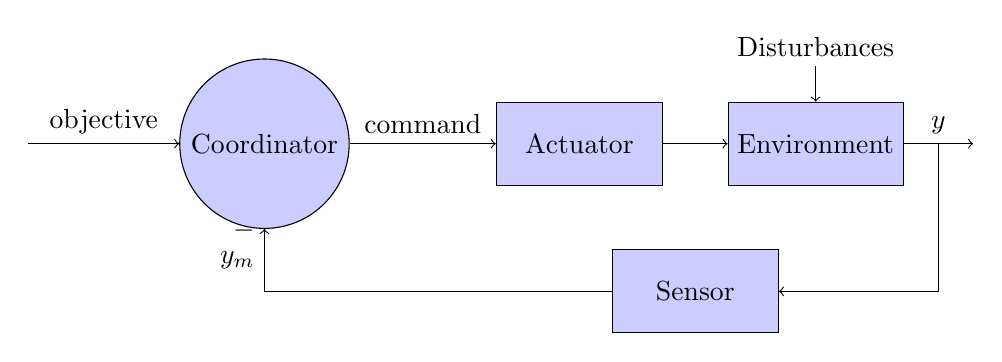
\begin{tikzpicture}[auto, node distance=2cm]
	% We start by placing the blocks
	\node [input, name=input] {};
	\node [sum, right of=input, node distance=3cm] (sum) {Coordinator};
	\node [block, right of=sum,  node distance=4cm] (controller) {Actuator};
	\node [block, right of=controller, pin={[pinstyle]above:Disturbances},
	node distance=3cm] (system) {Environment};
	% We draw an edge between the controller and system block to 
	% calculate the coordinate u. We need it to place the measurement block. 
	\draw [->] (controller) -- node[name=u] {} (system);
	\node [output, right of=system] (output) {};
	\node [block, below of=u] (measurements) {Sensor};
	
	% Once the nodes are placed, connecting them is easy. 
	\draw [draw,->] (input) -- node {objective} (sum);
	\draw [->] (sum) -- node {command} (controller);
	\draw [->] (system) -- node [name=y] {$y$}(output);
	\draw [->] (y) |- (measurements);
	\draw [->] (measurements) -| node[pos=0.99] {$-$} 
	node [near end] {$y_m$} (sum);
\end{tikzpicture}

\section{Sensors}

Sensors use the \textit{MQTT} protocol to send data to the coordinator via the MQTT Broker

\section{Actuators}
Actuators use the \textbf{CoAP} protocol to receive commands from the coordinator. They have also set their associated sensor in their configuration to close the control loop

\section{Coordinator}

\paragraph{}
The coordinator is the central \textbf{collector} of the IoT application, it's in charge of storing data in the database and controlling the various control loops, applying the various policies for each pair sensor, actuator.

\paragraph{}
It's implemented in \textit{Java} using Eclipse's libraries to interface it to MQTT and CoAP networks; in particular we've implemented several \textit{interfaces} to make the program easy to ready and to extend the logic to future sensors and actuators.



\section{Data encoding}

\chapter{Analytics}

\section{Database}

We're using a \textit{MySQL}-compatibile database management system, cllaed \textit{MariaDB}. We're storing historic sensors' data in tables, one for each sensor's class, in the form of tuples: timestamp, sensor's id and sensor's datum. The following \textit{DDL} was used to build the zoo's database:

\lstinputlisting[firstline=7,language=SQL]
{../ddl.sql}

\section{Grafana}

Our project incorporates a real-time monitoring and visualization aspect through the implementation of a Grafana dashboard. This powerful tool allows us to seamlessly access and monitor the data stored in our database, enabling us to gain valuable insights into the trends and patterns of the monitored parameters.

By leveraging Grafana, we have created a user-friendly interface that presents the data in a visually appealing and intuitive manner. The dashboard provides real-time updates, allowing zookeepers, administrators, and other stakeholders to stay informed about the current status of the monitored parameters at a glance. The ability to view data trends in real-time empowers decision-makers to respond promptly to any deviations or potential issues, ensuring swift and appropriate action is taken.

Furthermore, Grafana enables the visualization of historical data, providing a comprehensive view of the parameter trends over time. This capability is invaluable for performing in-depth analysis and identifying long-term patterns and correlations. By visualizing historical trends, zoo staff can gain insights into seasonal variations, identify potential stressors or triggers for animal behavior, and make informed decisions regarding habitat management and animal care protocols.

\end{document}          
